\documentclass[a4paper,10pt]{article}
 
\usepackage{fullpage}%
%\usepackage[francais]{babel}%
\usepackage[francais,american]{babel}%
\usepackage[latin1]{inputenc}%
\usepackage[T1]{fontenc}%
\usepackage[obeyspaces]{url} \urlstyle{sf}%
\usepackage{moreverb}%
\usepackage{palatino}%
\usepackage{graphicx}%
\usepackage{amssymb}%
\usepackage{pstricks}
\usepackage{capt-of}%
\usepackage{subfigure}% 
\usepackage{verbatimfiles}
\let\bfseriesaux=\bfseries%
\renewcommand{\bfseries}{\sffamily\bfseriesaux}

\renewcommand{\|}{\url|}


%\parskip=0.3\baselineskip \sloppy

\begin{document}

\title{Internship report\\\emph{Codmon: a source code monitoring tool}}

\author{Fran\c cois LESUEUR}

\date{\today}

\maketitle


\begin{abstract}

Testing a software during all its development is quite hard. We often test a functionality, and consider it to be functional forever, which is often false. Therefore, we are proposing an automatic testing framework called \emph{Codmon}. We will explain its specificities, and show its specialization to a software, \emph{Ibis}.

\end{abstract}



\begin{figure}[b]
  \centering
  \emph{I am very grateful to Henri E. Bal and Rob V. van Nieuwpoort for welcoming me in their team.}\\~\newline
  \emph{Vrije Universiteit - Amsterdam}
\end{figure}
                                                                                
\clearpage
~\clearpage

\section{The testing problem}

%\subsection{Why ?}

Developing a software inherently creates inconsistencies in it. Someone adds a functionality at \emph{t}, and some other one breaks this functionality at \emph{t'}, without willing to. Another problem is about performance, when you have some figures, and when a few months later, the performances seem to have suffered a severe breakdown. Software are extremely complex, and no one can think about all the consequences when he tweaks a setting, or changes something. In this context, it clearly appears that automatic testing would be a good point. Such testing should monitor functionalities as well as performance, in a convenient way, allowing the programmer to easily add a test and see when there are problems. It should be extensible, since you can not write a testing framework for each software. Finally, it should be fully automatized, reporting problems directly to the programmer. Moreover, the described framework is designed to be parallel-aware.

%\subsection{Previous works}

Some testing frameworks already exist. Usually, you have to add some information to your code and call the appropriate methods (\emph{JUnit}). But there are some problems with these. First, they are fully part of the software, and so have to be integrated, which causes some work and makes them unable to test initial steps as compilation. Then, since they are part of the software, they only have a local point of view, which can be better in some situations, but not all: they do not permit to check the ``outside'' state, and they are really hard to use in a parallel environment.

Codmon aims to provide an external point of view on all of this. It is designed to be installed \emph{outside} of the software, computing overall results. This way, it is able to manage compilation tasks, as well as \emph{parallel} functionality tests and benchmarking.

\section{Codmon: Design}

Codmon is meant to be a highly customizable framework for source code monitoring. This way, the core is fully generic, enriched by external plug-ins. The core of Codmon is responsible for the overall progress (\begin{sc}Fig.\end{sc} \ref{fig:general}). First, it makes a \emph{shot} of the current state of the monitored software, according to a configuration file containing \emph{sensors} description (\begin{sc}Fig.\end{sc} \ref{fig:sensor_attr}). A \emph{sensor} is composed of the \emph{job} command (\emph{wrapper} + \emph{cmd}), and of some attributes. Then, it adds all the performance values, called \emph{monitors}, to a database, and finally, it eventually triggers some alarms. We have chosen to print \emph{time-graphs} for performance benchmarking, since it is the most convenient way for the human to quickly view changes.


\begin{figure}
  \centering
  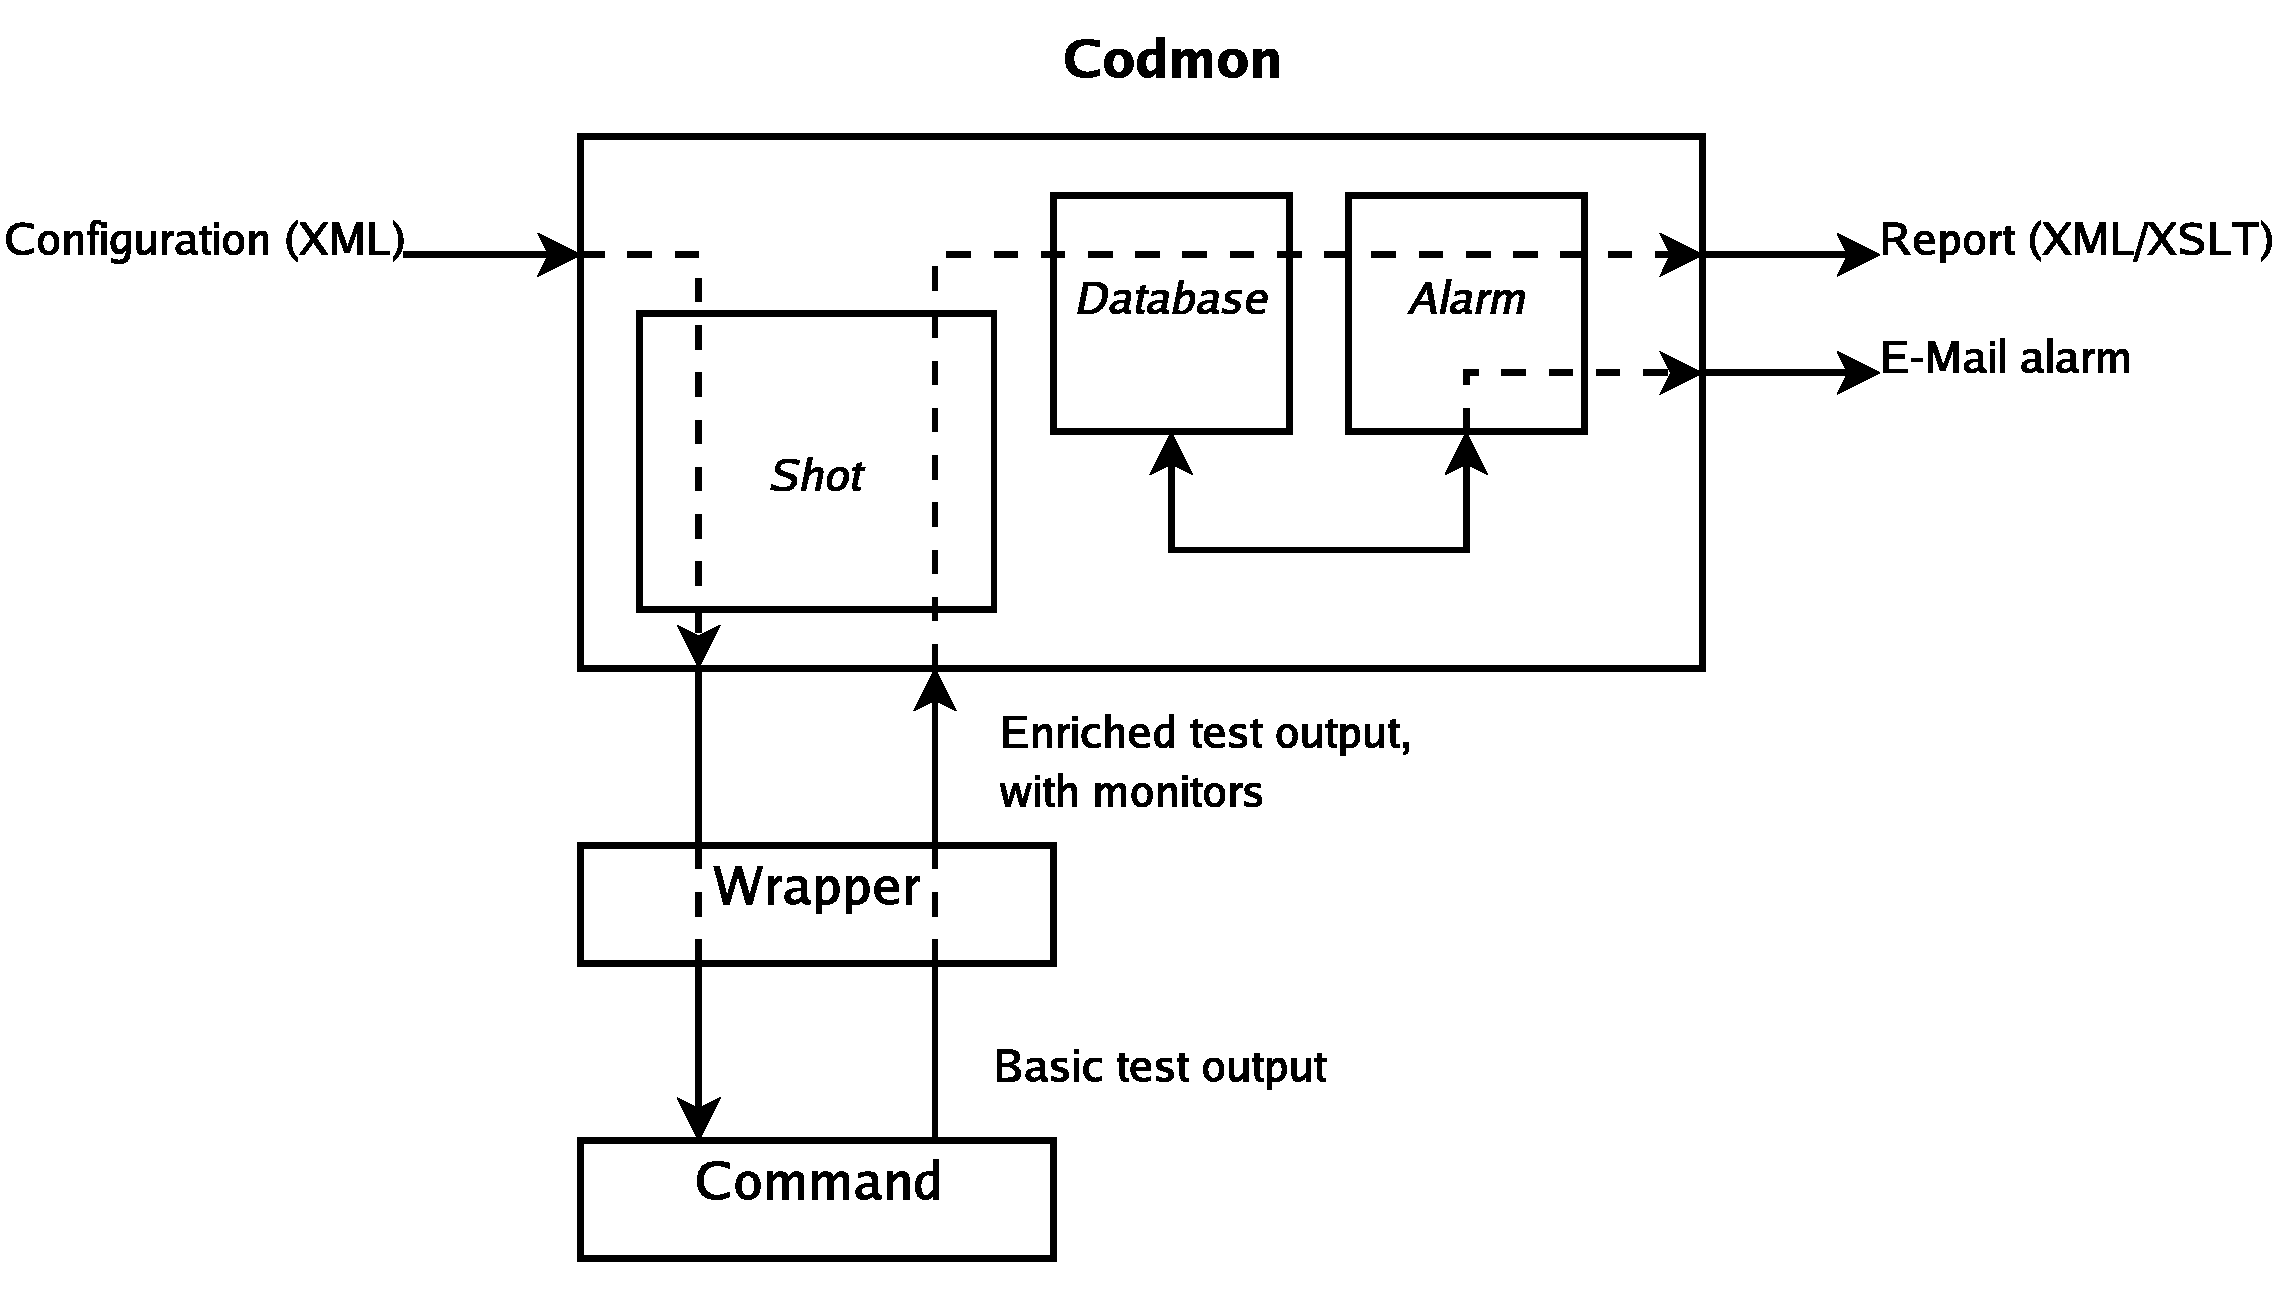
\includegraphics[width=\textwidth]{general}
  \caption{General design of Codmon's core}
  \label{fig:general}
\end{figure}


\begin{figure}[ht]
  \centering
    \subfigure[Common attributes]{
     % \begin{centering}
	\begin{tabular}{|r|l|} \hline
	  \emph{Attribute} & Meaning\\\hline
	  \emph{id} & Id of the sensor (must be unique)\\
	  \emph{name} & Name of the sensor\\
	  \emph{wrapper} & Wrapper to be used\\
	  \emph{cmd} & Command to be ran, eventually inside the \emph{wrapper}\\
	  \emph{scope} & The repository folder which should be analyzed in case of an alarm\\
	  \emph{scheduled} & Whether this sensor is scheduled\\
	  \emph{enabled} & Whether this sensor is enabled\\
	  \emph{fatal} & Whether failing in this step is fatal\\
	  \hline
	\end{tabular}
}
    \subfigure[Onoff additional attributes]{
     % \begin{centering}
	\begin{tabular}{|r|l|} \hline
	  \emph{Attribute} & Meaning\\\hline
	  \emph{graph} & Whether this sensor is to be graphed\\
	  \hline
	\end{tabular}
}
    \subfigure[Graph additional attributes]{
     % \begin{centering}
	\begin{tabular}{|r|l|} \hline
	  \emph{Attribute} & Meaning\\\hline
	  \emph{type} & ``throughput'' or ``latency''\\
	  \hline
	\end{tabular}
}
     % \end{centering}
   \caption{Sensor attributes}
  \label{fig:sensor_attr}
\end{figure}


\subsection{Core design}



The core executes a configuration file, describing the \emph{job} process to spawn and how to handle them. This file contains two main parts: a \emph{onoff} part, and a \emph{graph} part. The first one is used for compilation tasks and functional tests. The main result used is the return value of the spawned process. Such \emph{sensors} can also \emph{monitor} some events, but these graphs will not be analyzed for problems. Additionally to the return code, the \emph{error output} is also showed to the programmer. The \emph{graph} part is meant for benchmarks tasks. They are supposed to return some performance values, \emph{monitors}, as well as an effective return code. Alarms are triggered in case of a performance drop down or an execution error.

Each analyzed sensor has a \emph{scheduled} boolean attribute, which is true if the job is \emph{scheduled} downward (by a \emph{batch system} for instance). If set to true, jobs will be launched in parallel, letting the \emph{batch system} care about their real scheduling. If set to false, they are launched in a traditional, \emph{sequential} scheme. Job are merely supposed to go through \emph{wrappers}, which are the specialized, \emph{external} parts of Codmon. Codmon takes the return-value of the called job (which may have been piped through a \emph{wrapper}) as a success indicator (using Unix conventions, 0 being ``success'', other being ``failure''). If the job has failed, Codmon copies its error output for further analyzing. The process may also output \emph{monitor} information, which will be used in the next step.

After having launched all the jobs, Codmon updates its database with the new \emph{monitor} values. It then refreshes all the graphs. We chose to draw two graphs per monitor, a weekly one and a semester one. The weekly one is aimed at showing current problems, whereas the semester one is meant to show the overall progress. The database permits, if needed, to add some other graphs or to directly fetch some data.

Finally, there is a simple mechanism to trigger an eventual alarm. If a test returns a non-zero value, it of course raises an alarm. Concerning benchmarks, an alarm is raised in case there is a $r$ (currently $2/3$) performance drop down (with care of the type of data, \emph{throughput} or \emph{latency}). If an alarm is triggered, Codmon begins with sending an e-mail to the project supervisors, and to the last \emph{committers} in the \emph{scope} directory. The final report includes all tests, showing which ones were successful, disabled, or failed. In case of a failed test, the error output is written, as well as the last changed files in the \emph{scope} directory.

\subsection{Some wrappers}

As said before, Codmon is composed of a core framework, which is very generic, and some wrappers, which aim to provide some advanced functionalities. In this section, we are showing two example wrappers.

\subsubsection{Time wrapper}

This is the simplest wrapper. The aim is just to measure the execution time. It runs the job, and returns the job output plus the time elapsed.

\subsubsection{Outcmp wrapper}

This wrapper is somewhat a ``diff'' wrapper. It is aimed to compare the current output of a test to a \emph{referency} output. This way, we aim at detecting any malfunction, running errors as well as result errors. This is especially interesting in a computational test, in which the most important part is the value of the result. Moreover, since we are working in a parallel environment, we have no warranty about the order of the global output. The \emph{referency} file contains some lines to match, and the algorithm will just try to match them. Consequently, having more lines on the real output than on the \emph{referency} one is not considered as an error. Moreover, to handle the ``disordered'' output, we can group some lines, which generates a \emph{pool} of lines. Such \emph{pool} is matched \emph{in any order}. Finally, there is also a support for a global ``ignore file'', which contains patterns which are to be skipped on every output. Such patterns should cover non-static lines, as those printing a time value. This is just a shortcut to ease the creation of \emph{referency} output files.



\section{Codmon: Implementation}

Codmon has been implemented to monitor the \emph{Ibis project} (\|http://www.cs.vu.nl/ibis|). \emph{Ibis} is a middleware for \emph{grid-computing}, developed at the Vrije Universiteit (Amsterdam), and written in Java. It features some parallel output, as well as computation tasks, which make it a perfect test bench for Codmon. Its repository is managed through CVS. The Codmon philosophy is to provide a generic framework, and some really specific scripts to adapt it to \emph{Ibis}. The aim is to have a totally autonomous yet easy to maintain system, and portable to another software with little work.

\subsection{Core implementation}


The core has been written in Java. It reads a configuration file written in XML (\begin{sc}Fig.\end{sc} \ref{fig:xml_config}), using the DOM parser. The \emph{monitors} returned are XML nodes (\begin{sc}Fig.\end{sc} \ref{fig:xml_monitor}), and the process can return HTML code, enclosed in \emph{<html>} tags. We use the JRobin library (\|http://www.jrobin.org|) to handle the database and the associated graphs. It features a Java implementation of the RRDTools from Tobias Oetiker (\|http://people.ee.ethz.ch/~oetiker/webtools/rrdtool/|). It consists of a Round Robin Database, which takes care of discontinuities and dropping old values, and of the associated graph generator (\begin{sc}Fig.\end{sc} \ref{fig:graph}).\\
All the outputs (mail, final report) are written in XML, and transformed into HTML through different XSLT style-sheets (\begin{sc}Fig.\end{sc} \ref{fig:html} and \begin{sc}Fig.\end{sc} \ref{fig:html2}). This way, the output presentation as well as its ``medium'' is highly customizable. The eventual HTML parts of the jobs' outputs are rawly integrated into the final HTML.


\begin{figure}[ht]
  \begin{center}
    \begin{tabular}{|r|} \hline
      \begin{minipage}{\textwidth}
	\begin{tabbing}
	  iii\=iii\=iiiiiiiiiiiiiiii\=iii\=\kill\\
	  \texttt{<sensors>}\\
	  \>\texttt{<onoff>}\\
	  \>\>\texttt{<sensor id=''onoff\_id''}\\
	    \>\>\>\texttt{name=''Sample onoff sensor''}\\
	      \>\>\>\texttt{wrapper=''outcmp\_ibis''}\\
		\>\>\>\texttt{cmd=''2 ibis/apps/build Main''}\\
		  \>\>\>\texttt{scope=''ibis/src''}\\
		    \>\>\>\texttt{scheduled=''true''}\\
		      \>\>\>\texttt{graph=''false''}\\
			\>\>\>\texttt{enabled=''true'' />}\\
	  \>\texttt{</onoff>}\\
	  \>\texttt{<graph>}\\
	  \>\>\texttt{<sensor id=''graph\_id''}\\
	    \>\>\>\texttt{name=''Sample graph sensor''}\\
		\>\>\>\texttt{cmd=''make\_graph''}\\
		  \>\>\>\texttt{scope=''ibis/src''}\\
		    \>\>\>\texttt{scheduled=''true''}\\
			\>\>\>\texttt{enabled=''true'' />}\\
	  \>\texttt{</graph>}\\
	  \texttt{</sensors>}\\
	\end{tabbing}
      \end{minipage}\\
      \hline
    \end{tabular}
  \end{center}
  \caption{Sample XML Configuration: the ``Sample onoff sensor'' is a \emph{onoff} sensor. It will execute ``2 ibis/apps/build Main'' in ``outcmp\_ibis'', is associated with ``ibis/src'', may be run in parallel with other jobs, will not draw any graph, and is enabled. The ``Sample graph sensor'' is a benchmark sensor, which will simply execute ``make\_graph''.}
  \label{fig:xml_config}
\end{figure}


\begin{figure}[ht]
  \begin{center}
    \begin{tabular}{|r|} \hline
      \\
      \texttt{<test id=''test\_id'' name=''test name'' value=''356156452'' unit=''Bytes/s'' />}\\
      \\
      \hline
    \end{tabular}
  \end{center}
  \caption{Sample XML Monitor: this is a sample output of a ``graph'' sensor.}
  \label{fig:xml_monitor}
\end{figure}


\begin{figure}
  \centering
  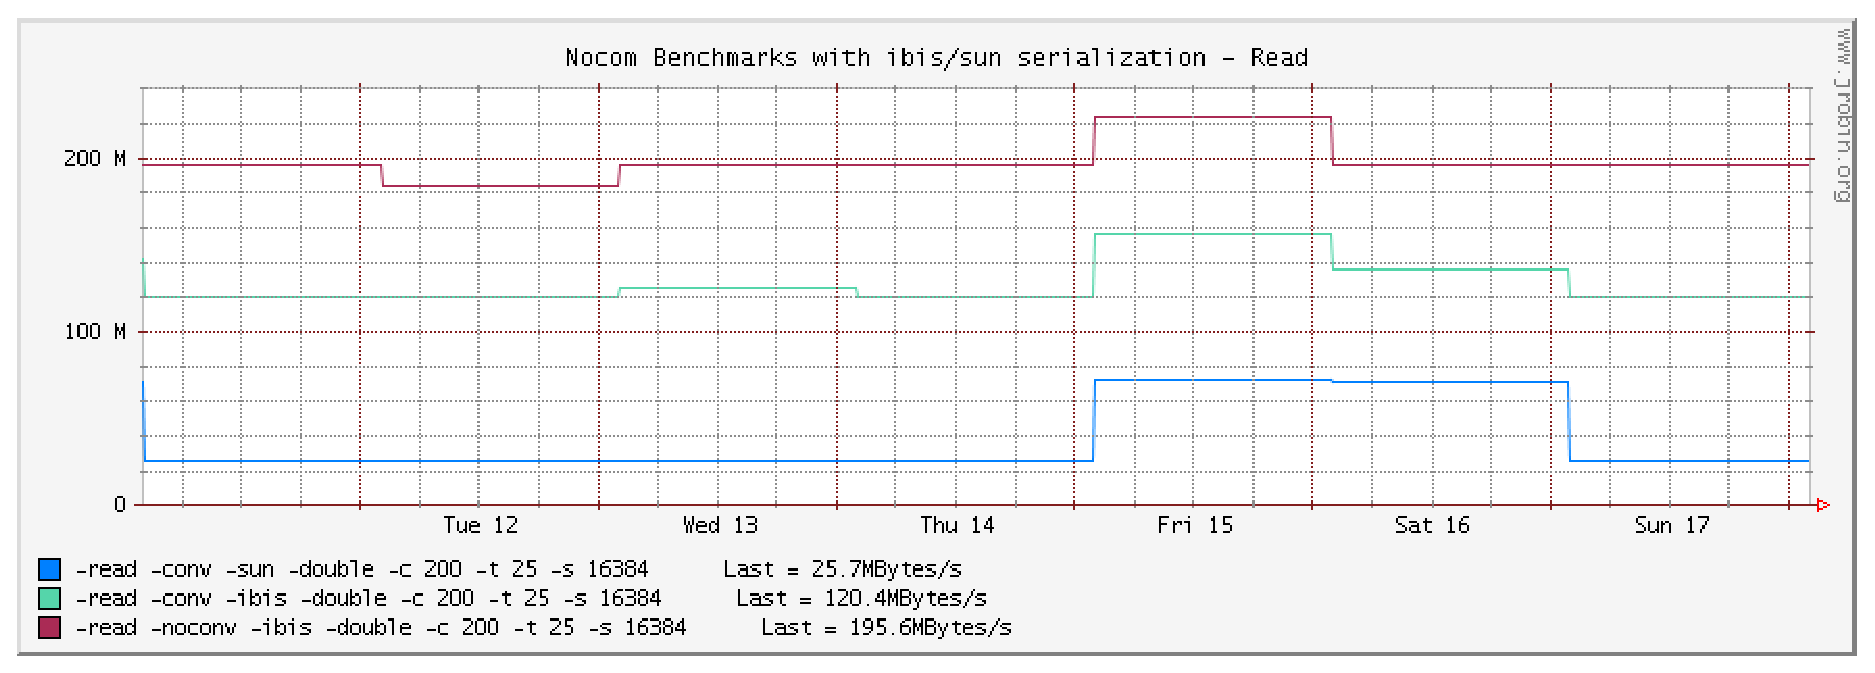
\includegraphics[width=\textwidth]{graph}
  \caption{Sample benchmark's graph}
  \label{fig:graph}
\end{figure}

\begin{figure}
  \begin{center}
    \begin{tabular}{|c|} \hline
      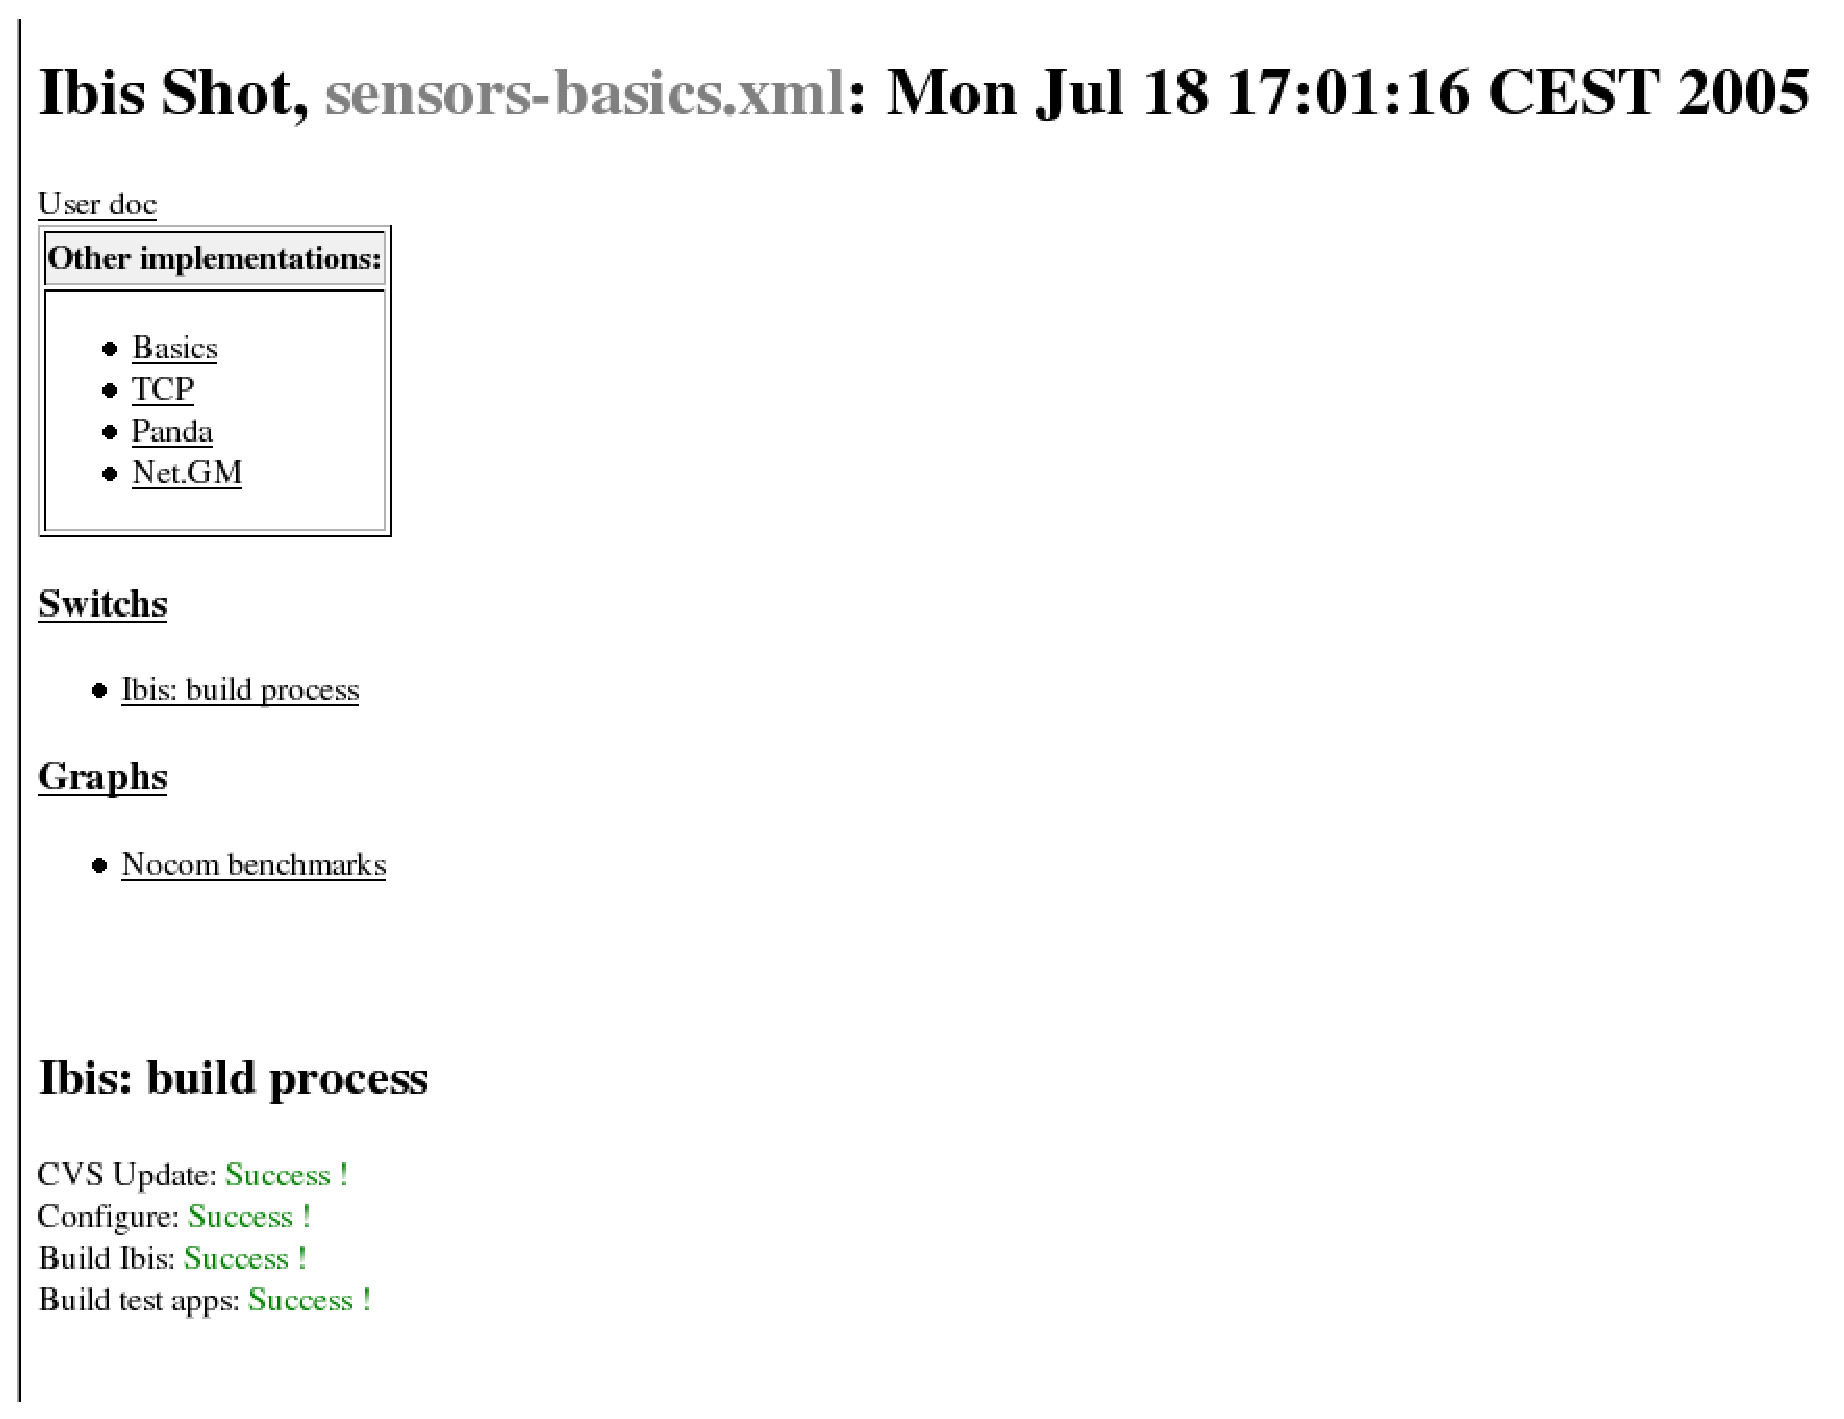
\includegraphics[width=\textwidth]{html}\\
      \hline
    \end{tabular}
  \end{center}
  \caption{Sample HTML output}
  \label{fig:html}
\end{figure}

\begin{figure}
  \begin{center}
    \begin{tabular}{|c|} \hline
      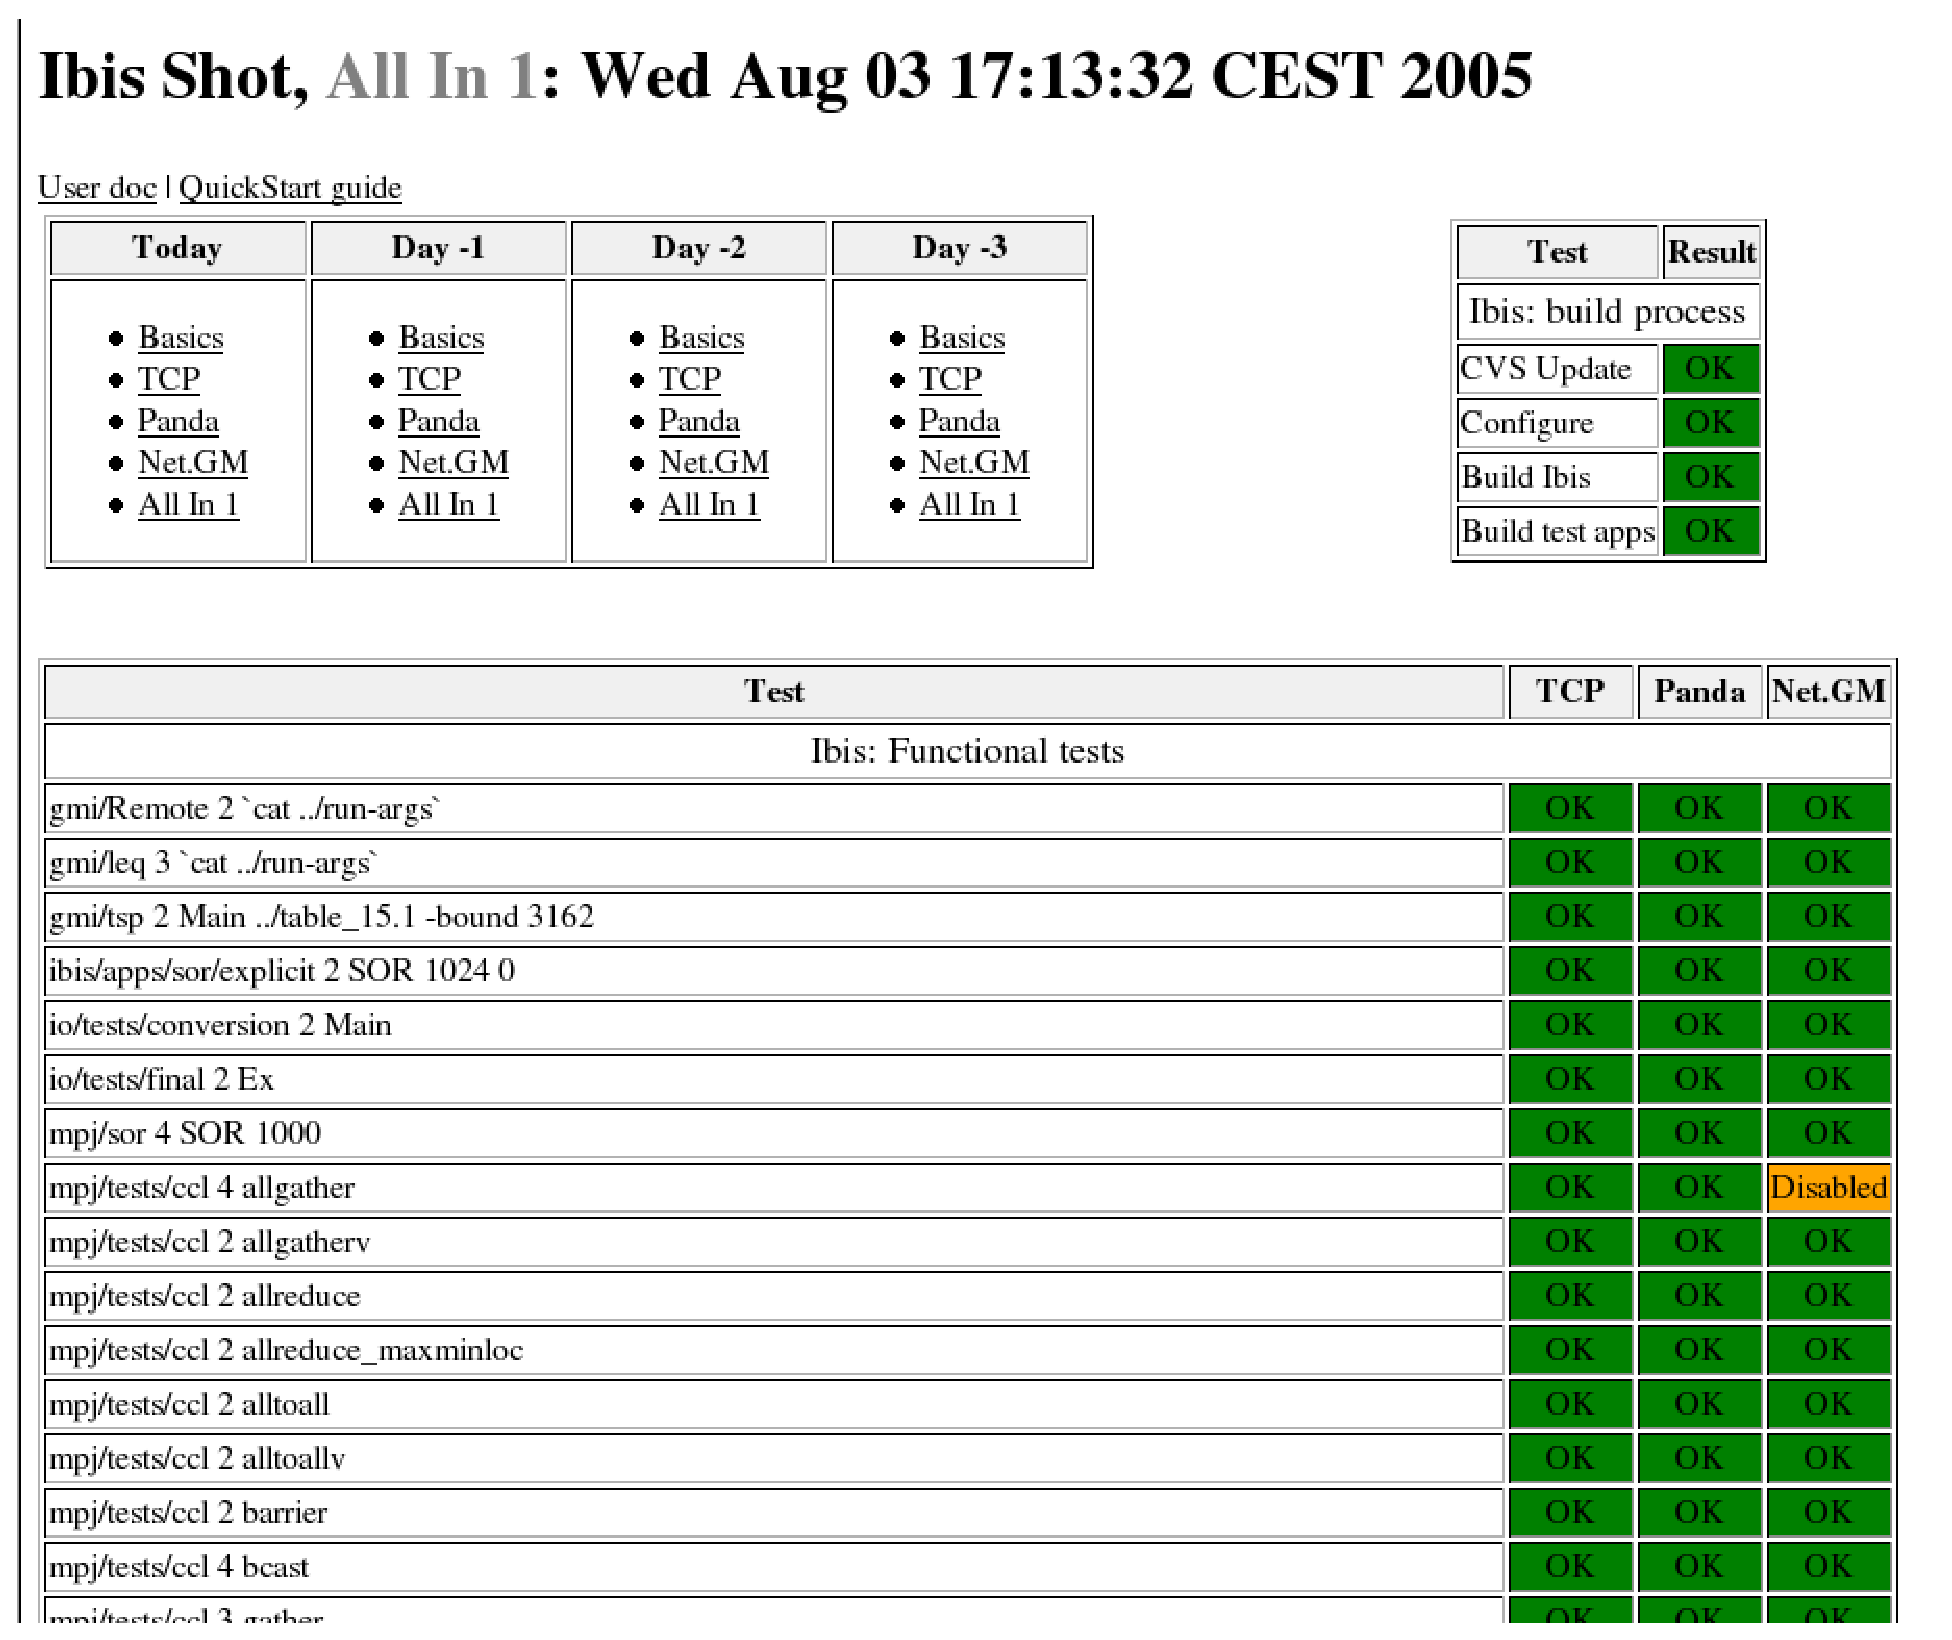
\includegraphics[width=\textwidth]{html2}\\
      \hline
    \end{tabular}
  \end{center}
  \caption{Sample HTML output, All In 1 view}
  \label{fig:html2}
\end{figure}


To ease the management of the different tests, we added an Ibis-specific script, written in Perl, gathering small configuration files and creating the global configuration (XML). These small configurations are handled in '.codmon' files, living in Ibis' applications directory. Since they all use the same wrapper, and since every job uses \emph{prun} (local batch system), we omit these parts in the '.codmon'. This way, every line contains only a few words: the number of nodes involved and the JVM run-args. We can temporarily disable some tests by preceding them of '//'. They will be part of the output, but marked as ``Disabled''. This is particularly useful when bug corrections are quite long, since this avoids developers being bothered by daily alarms for instance.

\subsection{Wrappers}

Wrappers are the interface between Codmon and the system. Therefore, they have to manage much parsing, and we chose to implement them in Perl. This is not a constraint: since they will be \emph{syscalled} by Codmon, every Unix program can be used as a wrapper. In this section, we describe the Outcmp wrapper, with its Ibis specificities.

This ``diff'' wrapper makes high usage of Perl regexps. It compares the current output of a command against a \emph{referency} file, which contains the expected return-value, STDOUT and STDERR. If this file doesn't exist, it creates it with the current output. Since we use Perl, the \emph{referency} file as well as the \emph{ignore-file} may include some regexps. The groups of unordered lines, \emph{pools}, are enclosed in '\{\}'. This wrapper returns a successful state as long as the output is as expected, which means that a non-zero return code from the test, if expected, can generate a successful state (useful for testing some ``exception'' tests).

In \emph{Ibis}, we use a specialized version of this wrapper. The \emph{referency} files are called '<Class name>.out.sample', and live in the application directory. They are part of the CVS tree, in order to provide users some sample outputs. If a new file has to be created by this script, it is automatically added to the CVS. This way, it is really very convenient for developers to manage Codmon, since they have direct access to these output files.

\subsection{Execution}

Codmon is launched by Cron on a daily basis. It first checks basic features (CVS checkout, \emph{Ibis} compilation, test applications compilation), then advanced features by running the whole set of \emph{Ibis} example applications. It outputs a few XMLs, related to different \emph{Ibis} implementations. The XMLs are served by an HTTP server, and are therefore accessible by any developer.



\section{Limitations and future works}

We now have a generic framework for source code monitoring. The major drawback are his \emph{genericity} and his \emph{straightforwardness}. First, being \emph{generic} enforces the developer to do some work to adapt it precisely to its needs. Therefore, due to the diversity of development systems (languages, tools, \ldots), it does not seem doable to do an ``universal'' testing software. We decided, instead of making a specialized one, to make a generic one which needs some specific code. The specific code is in fact an advantage.\\
Then, Codmon is quite \emph{straightforward}. It only runs specific commands, there is no support for some ``dynamic test''. For instance, with \emph{Ibis}, it might be interesting to run some tests on a variable number of nodes. Such feature needs some work to be \emph{cleanly} integrated, in a \emph{generic} way. Moreover, a little work could be done to allow an explicit refresh of a test.\\
Finally, there is no analysis of the system. A system change may broke some features on the monitored application. Currently, in this case, \emph{Codmon} will warn about an application problem, whereas the problem is related to the system. System change diagnostic is quite hard to make, though there is a first attempt to that in \emph{Diaspora} (\|http://projet.ifsic.univ-rennes1.fr/diaspora/|). The far future might be merging these two sides of analysis.


\section{Evaluation}

Codmon now runs for a little while on the \emph{Ibis} project. We decided to let Codmon create the \emph{referency} files of the \emph{Outcmp wrapper}, and then waited for errors to customize these files. With 150 tests, it took around 5 runs to have \emph{right} referency files. It has successfully detected some broken features, some of which were already broken \emph{before} the install of Codmon. Benchmarks are quite stable, and do not seem to trigger wrong alarms (which is hard to guarantee, since they can be disturbed).

One of the broken feature detected by \emph{Codmon} was in the \emph{MPJ} code. \emph{MPJ} is a module for Ibis, providing an \emph{Message Passing} interface for Java. Codmon showed some failures as soon as the \emph{-server} flag was passed to the JVM, which is a Sun-JVM option supposed to optimize the communication scheme for servers. Regarding that, the developer quickly thought about a race-condition in his code, and fixed it on the same day. We don't know how long this bug has lived in the \emph{MPJ} code, but what is sure is that this is \emph{Codmon} which permitted to reveal it.

\section{Conclusion}

We presented a source code monitoring framework, \emph{Codmon}, and its \emph{Ibis} specializations. It aims at warning the developers in case of a functional failure or of a performance drop down. It is a generic framework, which can be used by itself, but which is more powerful with some specific modules. A few modules, adapted to \emph{Ibis}, are part of the distribution as samples. It has been implemented in Java and Perl, using XML and XSLT technology, which should permit it to run on any *nix system.

By the time, it has proved to be easily manageable by developers, and quite efficient in detecting problems.


\section{Annex}
\subsection{Annex A: Developer documentation}
\verbatiminput{../dev}

\subsection{Annex B: User documentation}
\verbatiminput{../user}

\subsection{Annex C: QuickStart guide for Ibis}
\verbatiminput{../quickstart}

\end{document}
